\section{Firmware for ST devices}
%The most time-consuming part of the work has been the development of the firmware for ST devices. Despite of all the documentation and examples available on the internet, dealing with these platforms (including the BLE stack) required some in-depth study of the standards, of the implementation in the ST development environment and some trial and error to get the wanted features for the project. I've done different trials for each device, in some cases starting from scratch, in some cases starting from the available examples, exploring different possibilities and then choosing the best performing one for my goals.  
First of it all, I needed to replace the original firmware on the ST boards, applying the required modifications (for example, the data rate). Examples and documentation on the Internet have been a good starting point: then, thanks to a step-by-step approach, I wrote and built the final firmwares for all the boards, keeping in mind both the desired functionalities and the devices limitations. 

\subsection{ST BlueTile, sensing firmware}
The first board I've worked on has been the ST BlueTile one, because of its simpler configuration. In particular, I used the original firmware, called \textit{SensorDemo} \cite{bluetilesdk}, as a base for further development: in this way, the compatibility with the ST application is maintained.

The behavior of the base software is explained in Figure \ref{fig:bluetile-firmware}. It consists in a main loop, on the left part of the flowchart: at each execution, the value of some flag variables is checked and the corresponding event is executed. For example, if the variable \textit{imuTimer\_expired} is 1, it is reset and the value of the motion sensors is sent to the Bluetooth Low Energy stack for transmission. The value of these flag variables is set asynchronously by some interrupt procedures (in rectangles), that are triggered by specific events. For example, a set of hardware timers (Env Timer and Imu Timer) is configured to publish sensor and environmental data at specific rates, while other procedures will manage the behaviour at Bluetooth connection/disconnection. 

    \begin{figure}[ht!]
        \centering
        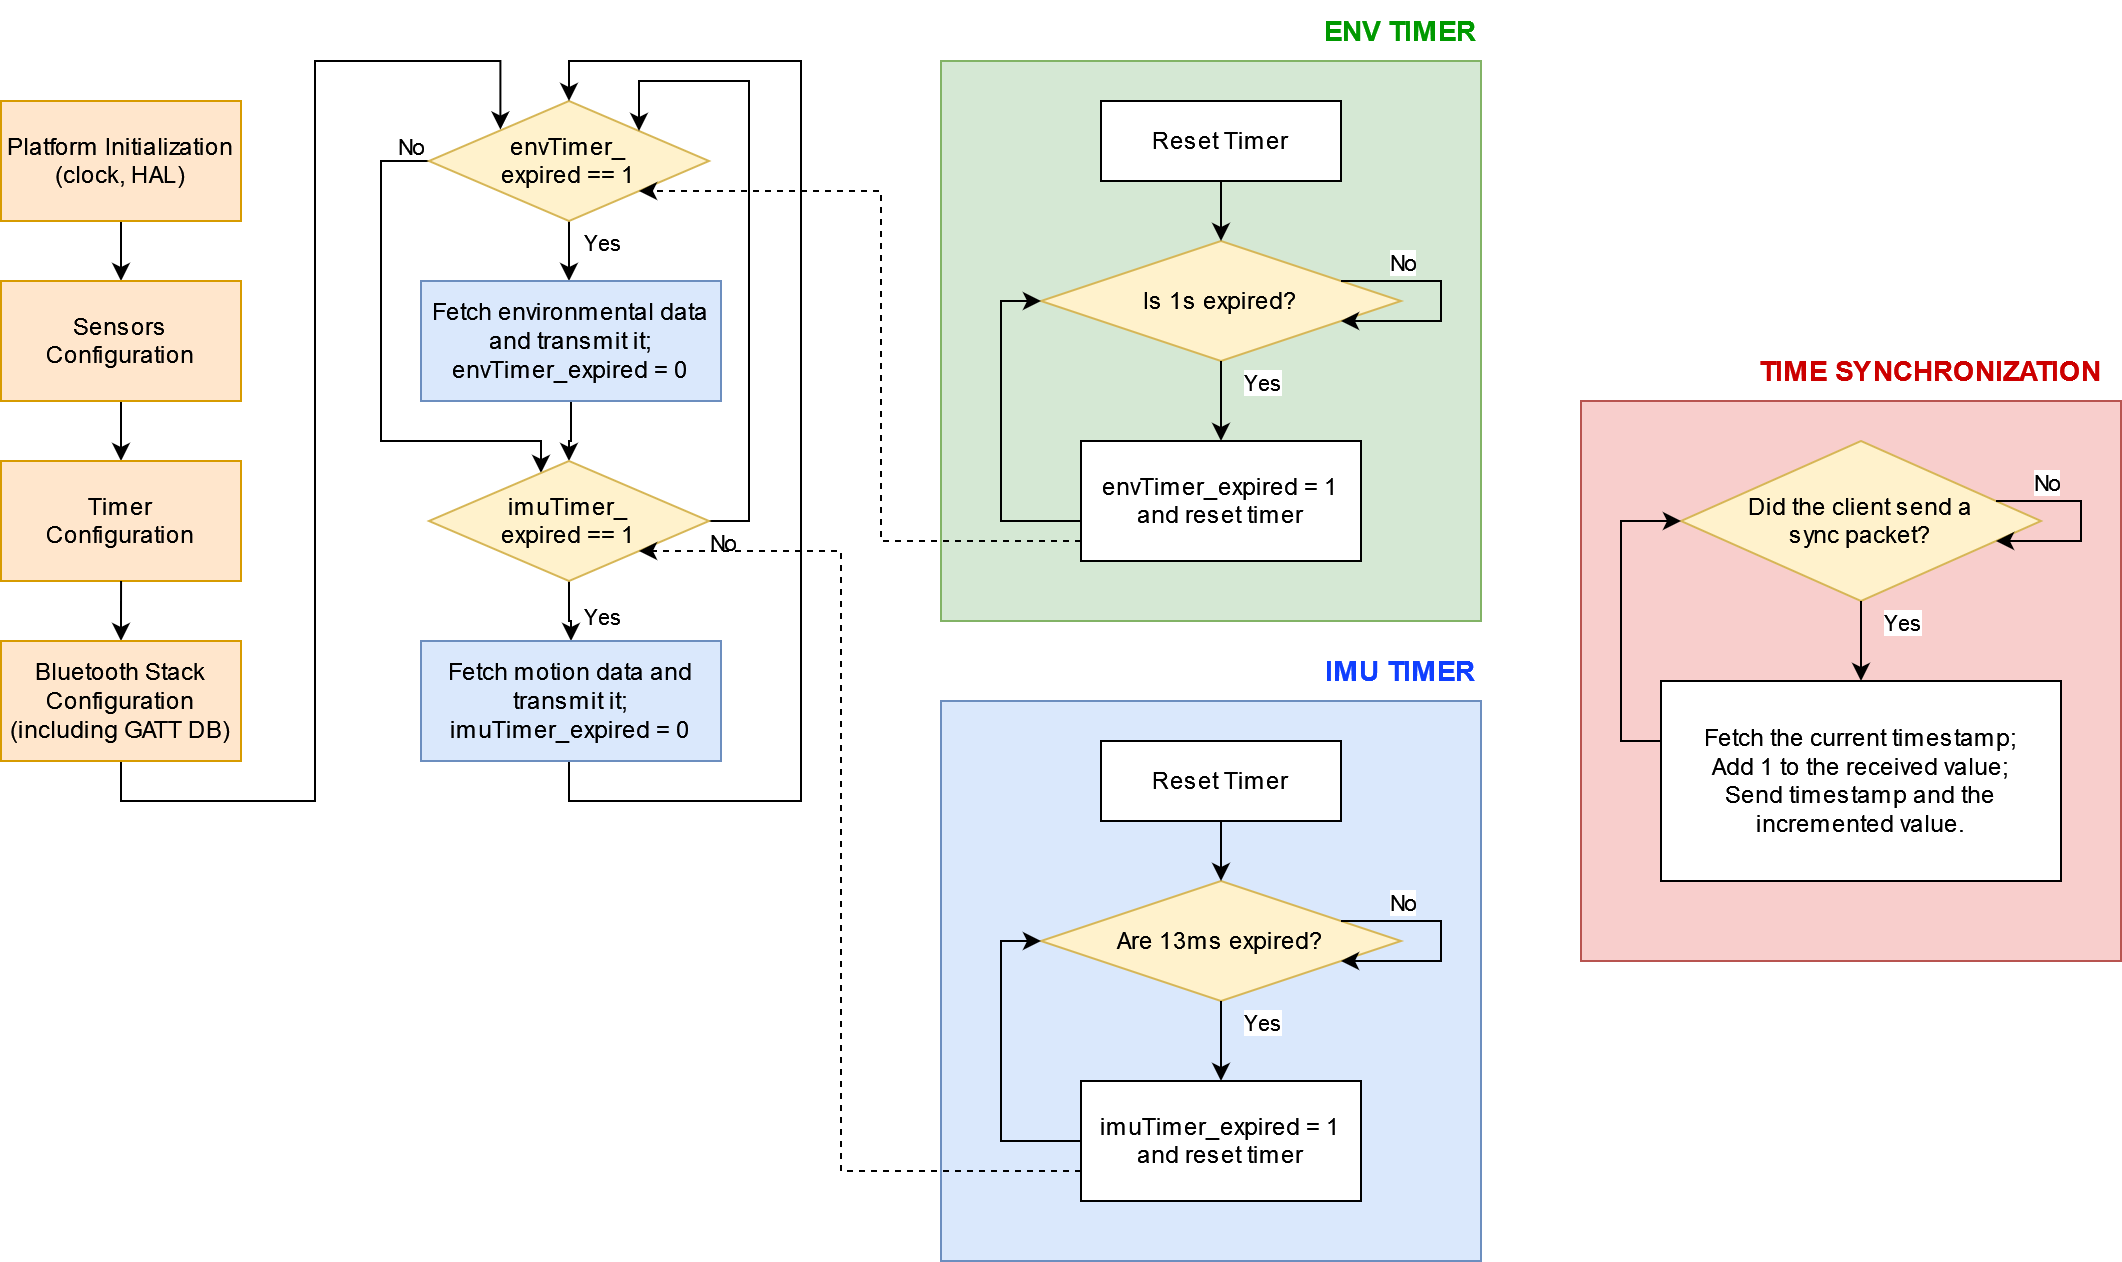
\includegraphics[width=0.85\textwidth]{chap3/figure/BlueTileFlow.png}
        \caption{Flowchart of the firmware for the BlueTile that streams sensor data.}
        \label{fig:bluetile-firmware}
    \end{figure}

The \textit{SensorDemo} firmware also contains the \textit{ST BlueVoice} library, that allows the streaming of compressed sound via Bluetooth Low Energy, optimized for voice transmission.  
I'm explaining the firmware functionalities in the following list, underlining the differences from the original one:
\begin{itemize}
    \item \textbf{Sensor data readings}. The information chosen to be transmitted to the client are the IMU (accelerometer, gyroscope, magnetometer), pressure, humidity and temperature sensors. 
    \item \textbf{Data rate modification}. I modified the rate at which IMU sensor data is transmitted over Bluetooth from 25~Hz to 75~Hz (in the last version of the firmware). Some intermediate tests have been done with other frequencies, in order to find the best one, with the corresponding results reported in the Results chapter. To perform this task, I modified the intervals of the timers which trigger sensor data updates accordingly. The rate for environmental sensor data has been lowered from 2Hz to 1Hz. 
    \item \textbf{Timestamping}. The sensor data is timestamped at the moment in which the sensor is read, and immediately before sending the packet to the BLE stack. The \textit{getTimestamp} function returns the number of milliseconds elapsed since the board power up.
    \item \textbf{BlueVoice disabled}. Even if no audio streaming is enabled, leaving \textit{BlueVoice} enabled on the small Cortex-M0 processor of the BlueTile causes some important performance degradation in sensor data streaming. This is due to some interrupts that are remaining active for audio data processing and, eventually, activation of the audio streaming functionality. For these reasons, I've commented out all the code relative to \textit{BlueVoice} initialization and processing.
    \item \textbf{Connection parameter update}. In order to enable the maximum possible throughput, as explained in the Background part, I set the Connection Interval parameter to 7.5ms. This value is the same one configured on all the other devices. 
    \item \textbf{Timer modification}. When battery-operated, a timer will shut down the device if no connection is performed before 20 seconds, for battery life purposes. As this is not useful for our application, I disabled the relative timer.
    \item \textbf{Time synchronization mechanism}. As the time synchronization system requires two-way communication between the server and the client, the GATT database of the device should be set accordingly: I therefore added a GATT characteristic that can be read and written. Moreover, I re-wrote the interrupt procedure that is called when the GATT characteristic is written, to implement the synchronization behaviour that I explain later.
\end{itemize}

\subsection{ST BlueTile, audio streaming firmware}
 While one of the two BlueTile board has been used to only stream sensor data at the maximum data rate possible, the other one has been used to only perform audio streaming, to take advantage of the onboard microphone and the \textit{BlueVoice} library from ST. Also in this case, I used as starting point the \textit{SensorDemo} firmware example, that already contains the library. 

     \begin{figure}[ht!]
        \centering
        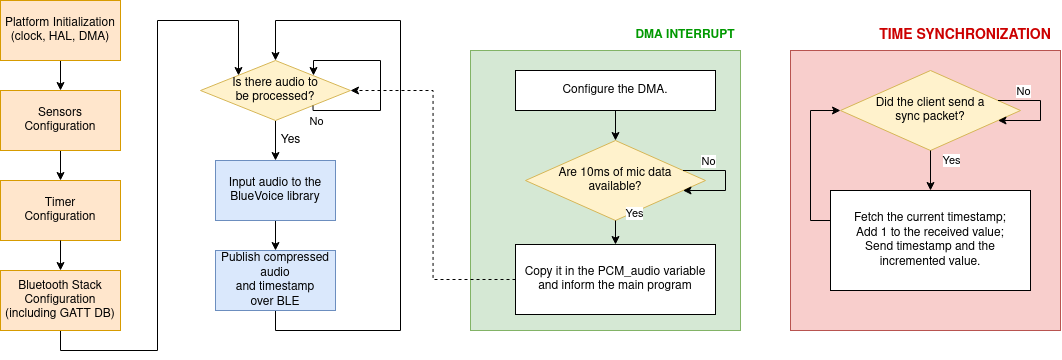
\includegraphics[width=0.85\textwidth]{chap3/figure/BlueVoiceFlow.png}
        \caption{Flowchart of the firmware for the BlueTile that streams audio data.}
        \label{fig:bluevoice-firmware}
    \end{figure}
 
 In this case, the resulting firmware is quite similar to the original one, with the modifications explained in the flowchart in Figure \ref{fig:bluevoice-firmware} and in following list:
 \begin{itemize}
     \item \textbf{Sensor Data Streaming}. I left the data rate of the sensors to the default value (25Hz). There is no necessity to fully disable the functionality from the firmware, because when voice streaming is active, the sensor data streaming is automatically disabled.
     \item \textbf{DMA configuration}. The microphone on the BlueTile board outputs data in the Pulse-Density modulation form (PDM): the frequency of ones is proportional to the sound pressure level. Usually, audio is represented using a different standard, called Pulse-Coded modulation (PCM), composed of 16 bits words ranging from 0 (no pressure) to \(2^{16}\) (maximum pressure). This conversion can be performed in hardware using the Direct Memory Access (DMA) component of the BlueTile SoC, that can asynchronously update the value of a variable (containing audio data) and then inform the main program through an interrupt. Hence, the DMA should be configured in the initialization phase to perform this operation.  
     \item \textbf{Timestamping}. The \textit{BlueVoice} library has been thought to stream audio information in real time, hence there was no need to timestamp the audio data. In my case, as this data is necessary for further analysis, there is the need to provide timestamps along with the audio samples. To do so, I added a GATT characteristic on which timestamping information is published. I also modified one of the \textit{BlueVoice} callback procedures, in particular the \textit{SendData} one, responsible of sending out samples once processed: just before publishing the audio data on its own GATT characteristic, the current timestamp is published on the other one. The client will then join them together.

     I put the implementation of this system in the separated \textit{timestamp\_helper.c} file, that contains the variables (GATT characteristic handle) and the two procedures (GATT characteristic creation, timestamp publishing) necessary for all of this to work.
    \item \textbf{Timer modification}. As done for the other firmware, I disabled the timer that automatically turns off the device after 20 seconds of inactivity if the device is battery-operated.
    \item \textbf{Time synchronization mechanism}. Also in this case, I modified the GATT database to introduce the time synchronization mechanism.
 \end{itemize}
 

\subsection{ST SensorTile.box firmware}
 The SensorTile.box presents some differences from the other device from ST. Even if the software stack is similar, there is no possibility to program the BlueNRG microcontroller, that is controlled by the STM32 Cortex-M4 processor, the only one accessible by the developer. This difference unlocks a great number of other possibilities, thanks to the computing power and the STM32 libraries, but the firmware development becomes a little more complex.
 
 The definitive solution consisted in using the \textit{ALLMEMS-1} firmware example from ST \cite{allmems1}, modifying it according to my needs. In this case, this software has been the best choice, as other ones didn't include support for some sensors like the microphone. It is worth noticing that the SensorTile.box presents no support for the \textit{BlueVoice} library, hence it is possible to extract information from the audio stream, but not to send it real-time to the client. 
 
 Finally, regarding the BLE stack, it is interesting that its abstraction layer is providing C functions working in the same way as they're working in the BlueTile, even if the hardware is quite different. As a consequence, full compatibility with parts of BlueTile firmware is assured: GATT characteristic creation/update, connection configuration, callback procedures all work in the same way. The final firmware is represented in Figure \ref{fig:sensortilebox-firmware}.

      \begin{figure}[ht!]
        \centering
        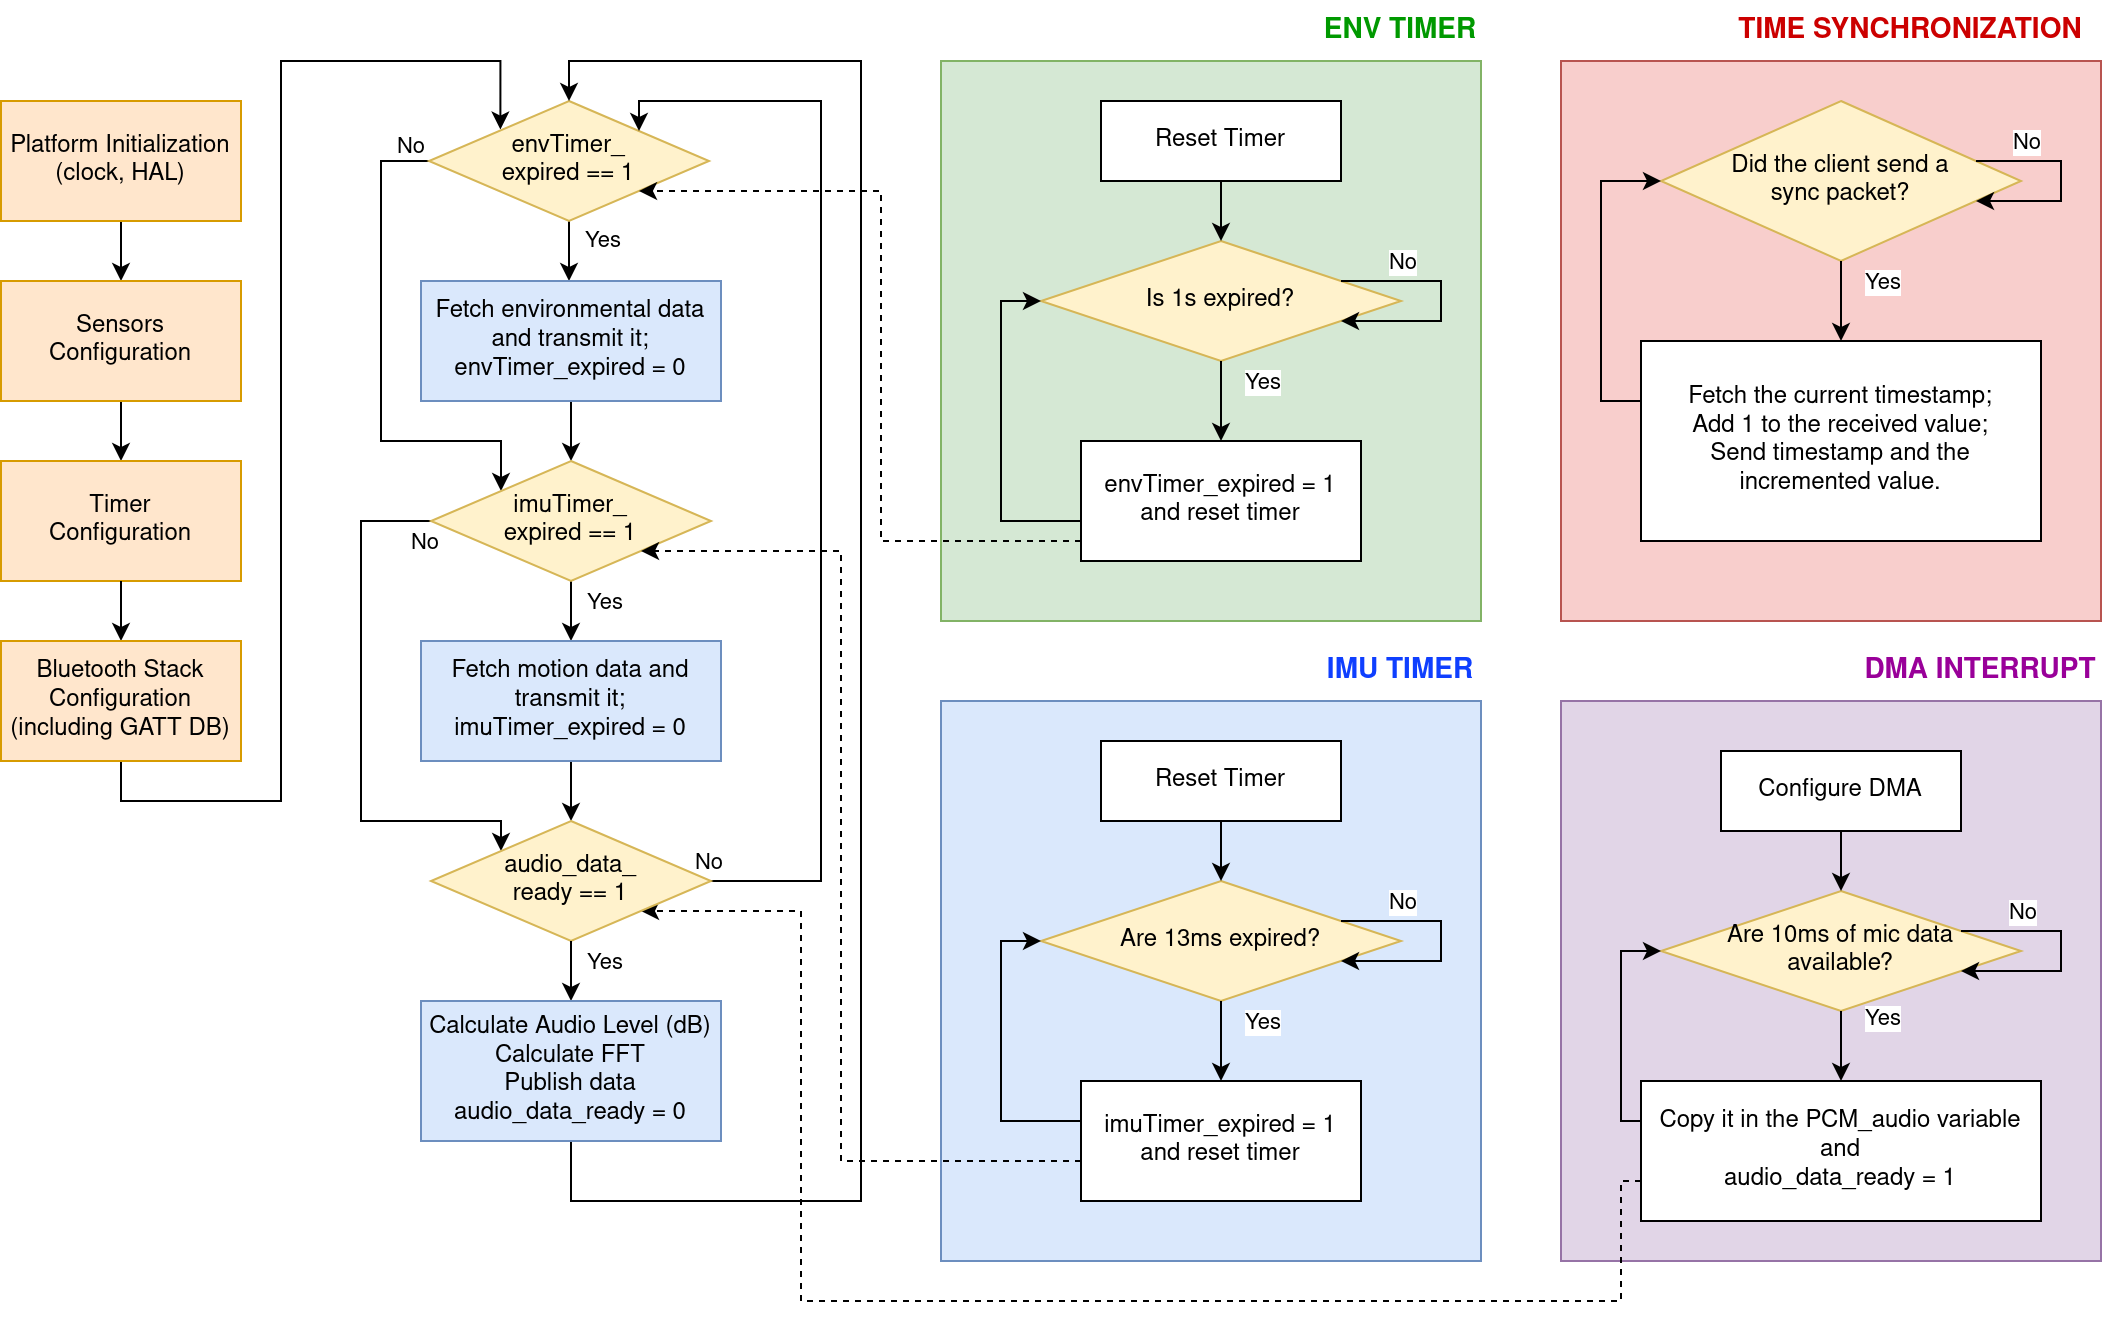
\includegraphics[width=0.85\textwidth]{chap3/figure/STbox.png}
        \caption{Flowchart of the firmware for the SensorTile.box.}
        \label{fig:sensortilebox-firmware}
    \end{figure}

The following list explains the functionalities of the firmware and the work I've done on it:
\begin{itemize}
    \item \textbf{Sensor data streaming}. The information chosen to be transmitted to the client are the IMU (accelerometer, gyroscope, magnetometer), pressure, humidity and temperature sensors. 
    \item \textbf{Data rate modification}. Like what's has been done on the BlueTile, I modified the motion sensors data rate to 75Hz and environmental sensors data rate to 1Hz, setting accordingly the timer variables. 
    \item \textbf{Timestamping}. The timestamping on the SensorTile.box firmware had a different behaviour from the BlueTile one. It would still send the number of milliseconds elapsed from power on, but the three LSBs were shifted out and not sent to the client. To create consistency between devices and add precision (we need time to be as accurate as possible), I disabled the shifting, to transmit the entire timestamp. 
    \item \textbf{Time synchronization mechanism}. Also in this case, I modified the GATT database to make the time synchronization mechanism possible. 
    \item \textbf{Audio processing}. One of the interesting features of the SensorTile.box is the presence of a digital microphone. The ALLMEMS firmware from ST leverages this component offering the streaming of audio level information (in dB). To enrich the details on the surrounding audio, I added the information on the dominant frequency: the samples used to extract the dB information are also input for the \textit{arm\_rfft\_fast\_f32} function from the Common Microcontroller Software Interface Standard (CMSIS) from ARM, that is a a vendor-independent abstraction layer for microcontrollers that are based on ARM Cortex processors. For my use case, it provides an easy way to take advantage of the DSP included in the Cortex-M4 core available on the board. After getting the discrete real Fast Fourier Transform (FFT), the maximum magnitude for each output value is extracted, and the corresponding frequency index is sent on its own GATT characteristic, that I configured before.  
    I would like to underline that, also in this case, the configuration of the DMA has been necessary (as explained in the BlueTile chapter). 
    \item \textbf{Removing undesired functionalities}. The ALLMEMS firmware contains a lot of libraries from ST, used for sensor fusion and feature extraction (activity, gesture, position recognition and so on). To save battery, space and computational power (the FFT operation is pretty intensive), I disabled all these functionalities by commenting out their initialization code lines, along with the relative callback functions.  
\end{itemize}

